\section{Introduction}
This project is about the creation of a \textit{Miosix} driver for the ultrasonic distance sensor HCSR04 using hardware timers. 
\subsection{Problem statement}
The sensor HCSR04 is one of most used ultrasonic distance sensor in DIY projects due to its low retail price. Moreover it has features that make it a good alternative for simple applications. Some of its characteristics are:
\begin{itemize}
\item 0,02m-4m range;
\item 0.3 cm resolution;
\item quiescent current <2mA;
\item working current ~15mA.
\end{itemize}  
The aim of this project is to develop a driver for \textit{Miosix} operating system to allow developers to interface easily with this sensor.
\subsection{Summary of the work}
The driver uses hardware timer input capture mode to convert sensor answer into numbers representing the distance. The work has been divided in two main phases:
\begin{enumerate}
\item Understand how hardware timers work and how to use inpute capture to convert sensor answer;
\item Implement the driver for \textit{Miosix} operating system.
\end{enumerate}

\pagebreak

\section{Design and implementation}
\subsection{How the sensor HCSR04 works}
\begin{minipage}{0.5\textwidth}
The sensor has 4 pins:
\begin{itemize}
\item VCC: 5V Supply; 
\item TRIGGER: Trigger Pulse Input;
\item ECHO: Echo Pulse Output;
\item GND: 0V Ground.
\end{itemize} 
\end{minipage}
\begin{minipage}{0.5\textwidth}
\begin{figure}[H]
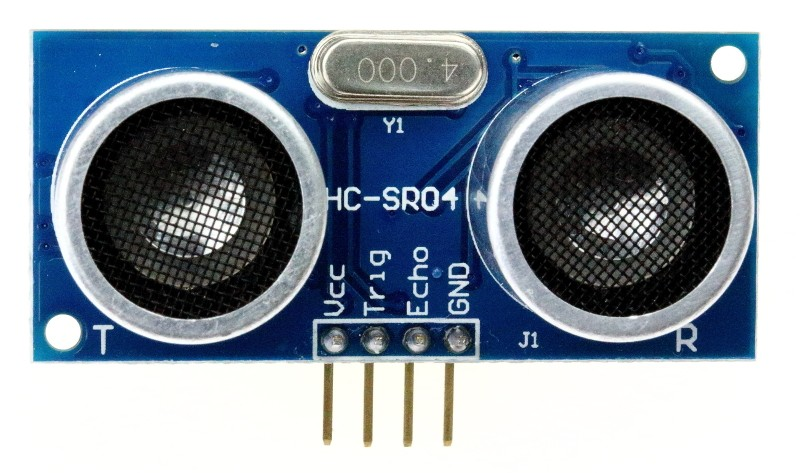
\includegraphics[width=\textwidth]{figures/raster/HCSR04}
\caption{\label{fig:sensor} HCSR04 sensor}
\end{figure}
\end{minipage} \hfill \\[1cm]

The basic principle of work consist of these steps:
\begin{enumerate}
\item Drive high level signal to TRIGGER pin for at least 10us;
\item The module sends eight sound bursts  at 40 kHz and detect whether there is a
pulse signal back;
\item The module drive the ECHO pin to high level signal for as much microseconds as the time the sound wave has traveled. 
\end{enumerate} 
\subsection{Class design and implementation}
The initial idea was to implement a singleton class but this would have limited the number of sensor that can be connected at the same time to one.
For that reason the class has been implemented as a multiton class where the instances created are stored into a static Map, using the number of the timer that the sensor uses as key. With this solution it's possible to connect up to 3 sensors.\\
The class \textit{hcsr04} has two public methods(both are thread-safe):
\begin{description}
\item [hcsr04* getInstance(int \textunderscore timer)] This function is called to return an instance of the class depending on the timer chosen,if no instance, that use that timer, exists it will be created. If the \textit{ \textunderscore timer} is not equal to the number of any of timer supported (3,4,5) the function returns NULL.
\item [float getDistance()] Function used to retrieve distance read by the sensor. To avoid interferences between measurements calls have to be spaced by at least 50-60ms
\end{description}

To make the sensor works, the driver, when create an instance of the class, sets the chosen timer CH1 and CH2 in input compare mode(both with TI1 as input) making the former channel sensible to raising edge and the latter sensible to falling edge. 
When the function \textit{getDistance()} is called this is what happens:
\begin{itemize}
\item 10us pulse is generated by software on TRIGGER pin and wait for sensor answer;
\item ECHO pin is driven to a high logic level by the sensor and a first interrupt is raised (CH1 detect raising edge);
\item The interrupt handler function enable the timer and the timer start to count;
\item When the sensor drive the ECHO pin to low logic level another interrupt is raised (CH2 detect falling edge);
\item Now CCR2 contains the sound travel time, expressed in microseconds, to obtain the distance CCR2 values is multiplied by 0.0343 and divided by 2.
\item The obtained distance is retrieved.
\end{itemize}

\section{Experimental evaluation}


\subsection{Experimental setup}
\subsubsection{Hardware setup}
The experimental test has been carried out connecting the HCSR04 sensor to a simple circuit realized on a stripboard and using the STM32F407vg Discovery board.\\
The circuit contains, besides the HCSR04 sensor, 3 led of diffent color (1 green, 1 yellow and 1 red) that will be turn on depending on the distance read by the sensor (there is no need to use resistor to limit current trough leds because GPIO pins output current is limited to 6mA) and a 10uF electrolytic capacitor placed between GND and VCC sensor pins that stabilizes VCC voltage and makes the sensor measurements more precise.\\[2.5cm]
\begin{minipage}{0.5\textwidth}
\begin{figure}[H]
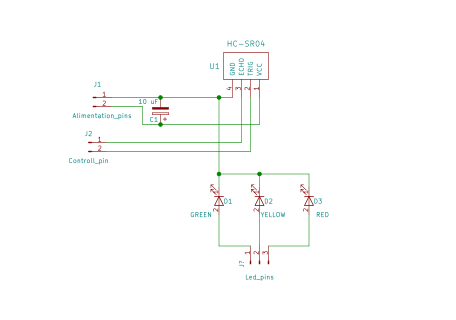
\includegraphics[width=\textwidth]{figures/raster/schematics}
\caption{\label{fig:sensor} Circuit schematics}
\end{figure}
\end{minipage}
\begin{minipage}{0.5\textwidth}
\begin{figure}[H]
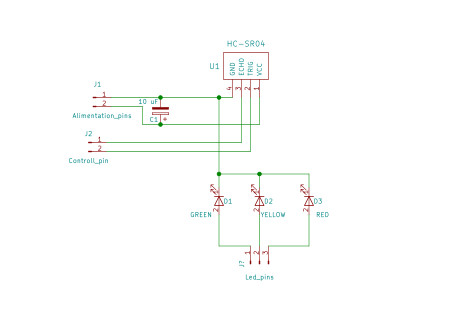
\includegraphics[width=\textwidth]{figures/raster/circuit}
\caption{\label{fig:sensor} Circuit realized}
\end{figure}
\end{minipage} \hfill
\newpage
\subsubsection{Software setup}
The code loaded on the board perform 100 distance reads and print the results on a serial port.
\lstset{language=C++,
                basicstyle=\tiny,
                keywordstyle=\color{blue}\ttfamily,
                stringstyle=\color{red}\ttfamily,
                commentstyle=\color{green}\ttfamily,
                morecomment=[l][\color{magenta}]{\#}
}
\begin{lstlisting}

#include <cstdio>
#include <miosix.h>
#include "hc-sr04.h"
#define TEST 100
using namespace std;
using namespace miosix;

typedef Gpio<GPIOB_BASE,2>  yellow;
typedef Gpio<GPIOE_BASE,8> red;
typedef Gpio<GPIOB_BASE,0> green;



int main()
{
	
    
   hcsr04 *sensor=hcsr04::getInstance(3);
    {
    	FastInterruptDisableLock dLock;
    	green::mode(Mode::OUTPUT);
    	yellow::mode(Mode::OUTPUT);
    	red::mode(Mode::OUTPUT);
    }
    
    for(int i=0;i<TEST;i++)
    {
    
   	
	float space = sensor->getDistance();
	
	printf("%.1f\n",space);
	if(space>=0.0 && space<50.0)
		{
			red::high();
			yellow::high();
			green::high();
		}
	else if(space>=50.0 && space<150.0)
		{
			red::low();
			yellow::high();
			green::high();	
		}	
	else
		{
			green::high();
			red::low();
			yellow::low();
		}
	sleep(0.5);
    }
  
  return 0;
  
}



\end{lstlisting}
\newpage
\subsection{Tests}
To verify if the driver works and how accurate is the sensor, the STM32F407vg Discovery board has been connected to the circuit created and to a laptop as follows:
\begin{itemize}
\item GND circuit pin to GND board pin;
\item VCC circuit pin to 5v board pin;
\item ECHO circuit pin to PC6 board pin;
\item TRIGGER circuit pin to PC7 board pin;
\item Green led to PB0 board pin; 
\item Yellow led to PB2 board pin;
\item Red led to PB8 board pin;
\item Board to laptop using a USB to TTL serial cable connected to USART3.
\end{itemize}

The measurements have been made placing the sensor 48 cm from the floor and putting an hard object (105 cm tall and 35 cm wide) at various distances. All the data have been logged by the laptop and, in a second moment elaborated, with \textit{Matlab}.\\
The tests do not consider scenarios where the object is moving, because, if the object is moving too fast, the sensor could not detect the object or retrieve a wrong value, or when the object is made by a soft material it can absorb part of the ultrasonic waves and alter the measure. 


\subsection{Results}
\begin{figure}[H]
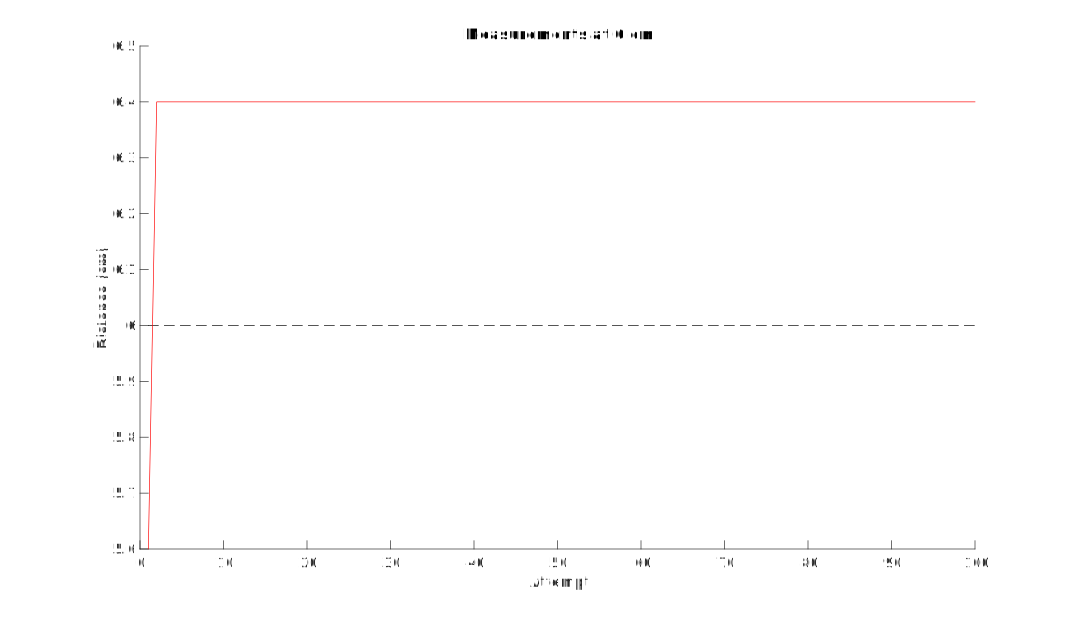
\includegraphics[width=\textwidth]{m6}
\end{figure}


\begin{figure}[H]
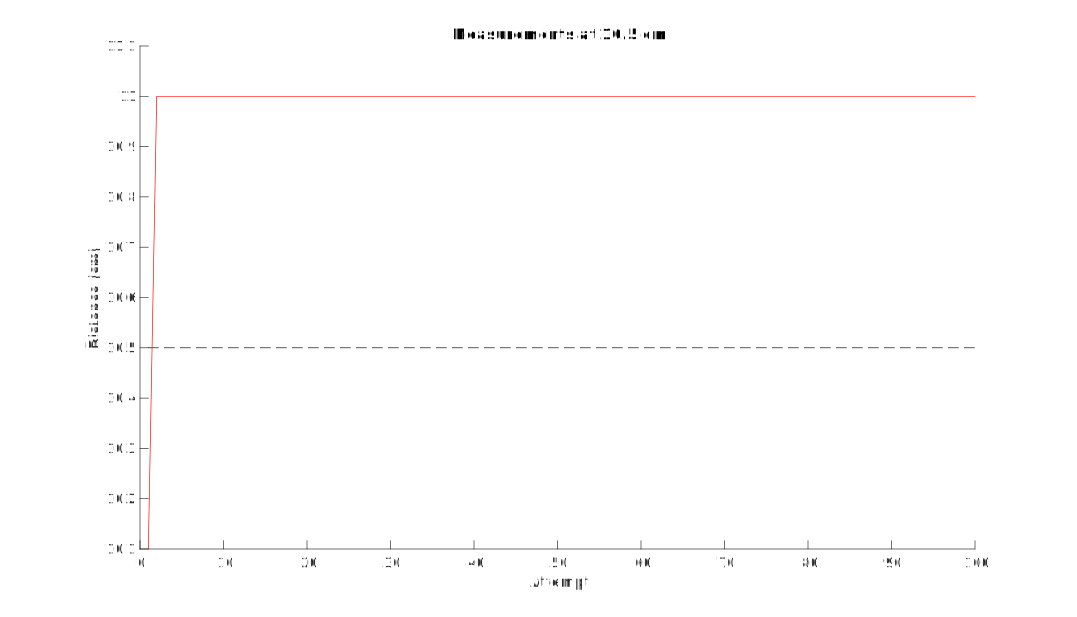
\includegraphics[width=\textwidth]{m10}
\end{figure}
\begin{figure}[H]
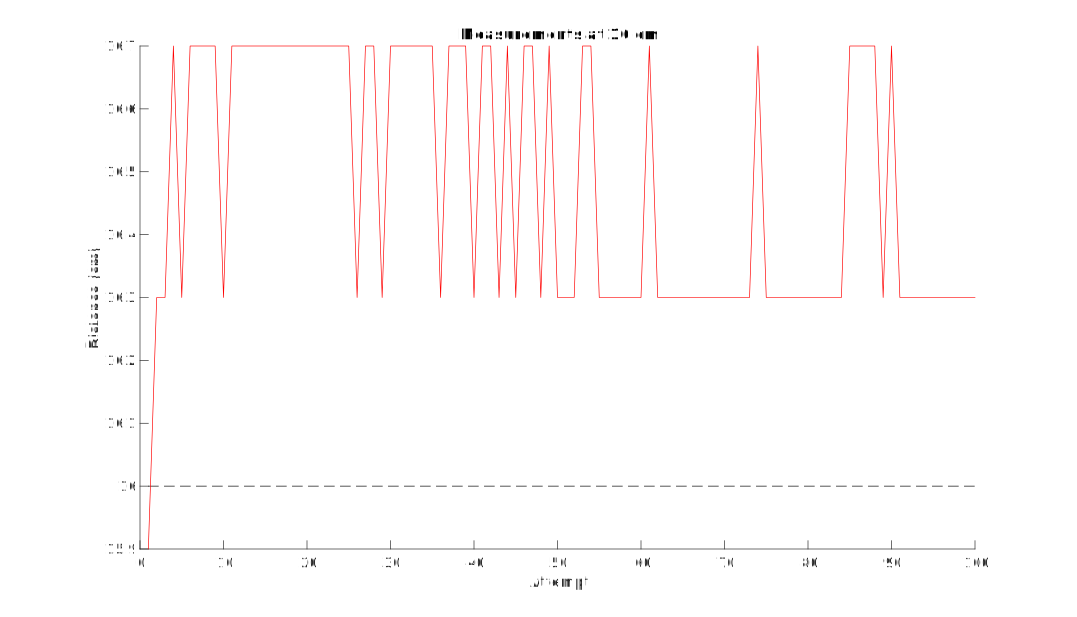
\includegraphics[width=\textwidth]{m16}
\end{figure}
\begin{figure}[H]
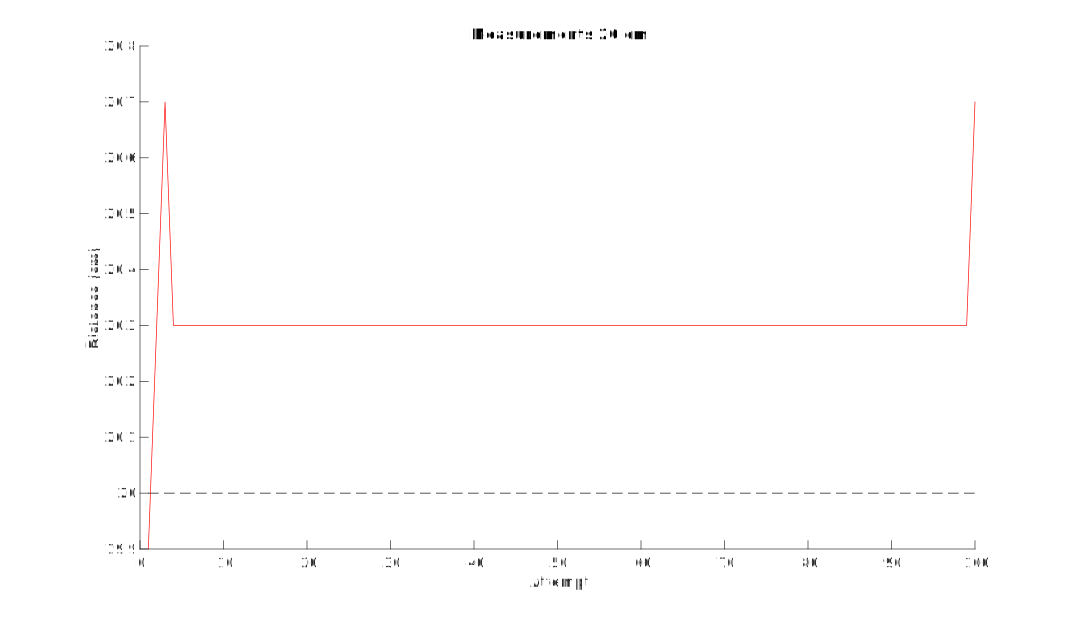
\includegraphics[width=\textwidth]{m20}
\end{figure}
\begin{figure}[H]
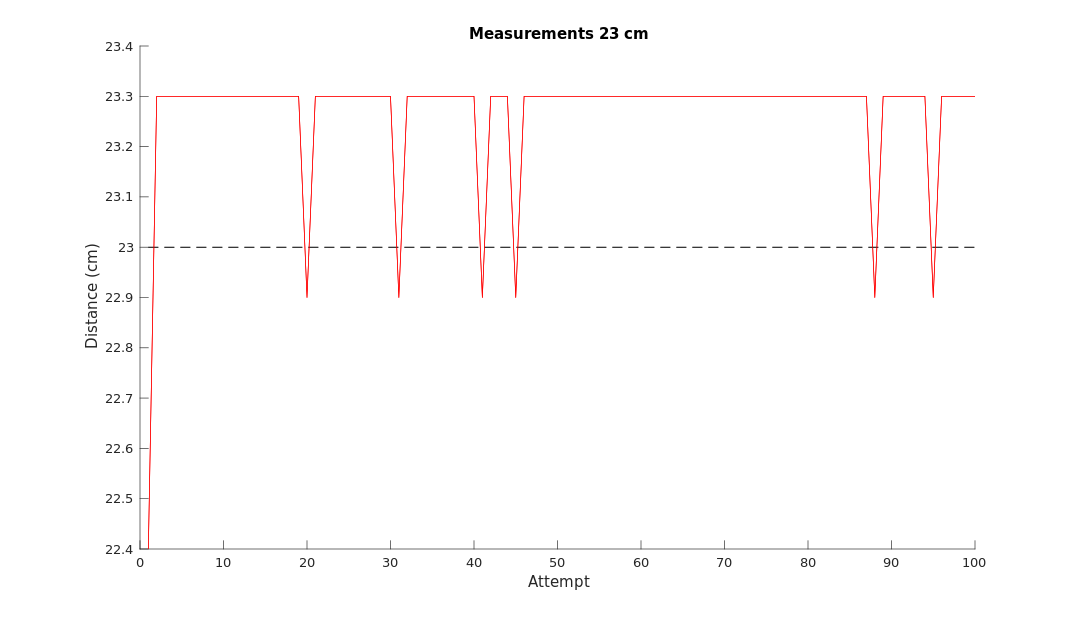
\includegraphics[width=\textwidth]{m23}
\end{figure}
\begin{figure}[H]
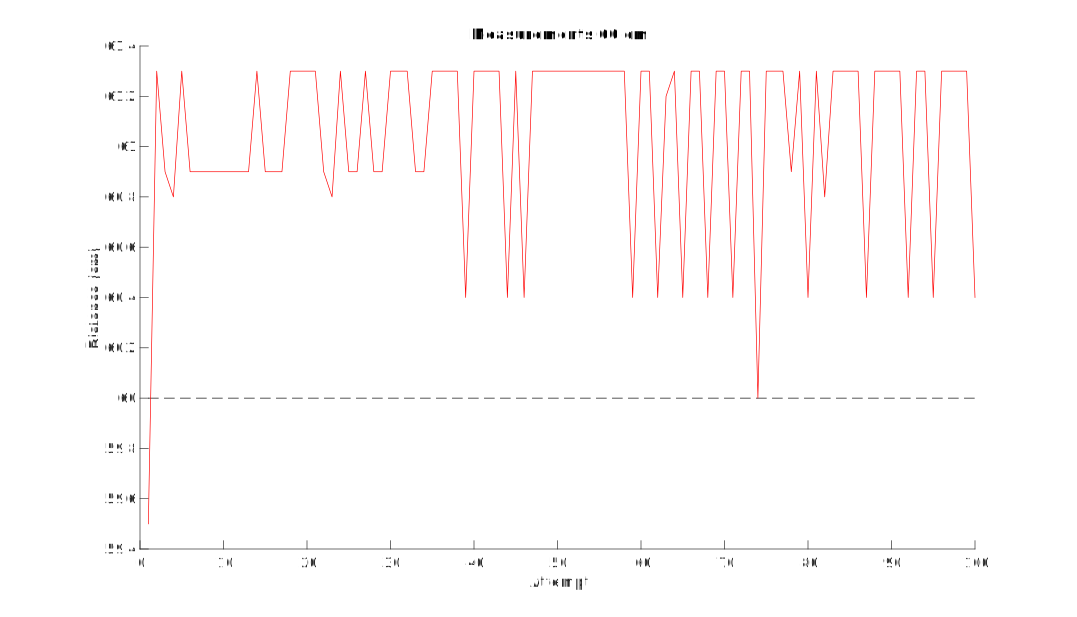
\includegraphics[width=\textwidth]{m60}
\end{figure}
\begin{figure}[H]
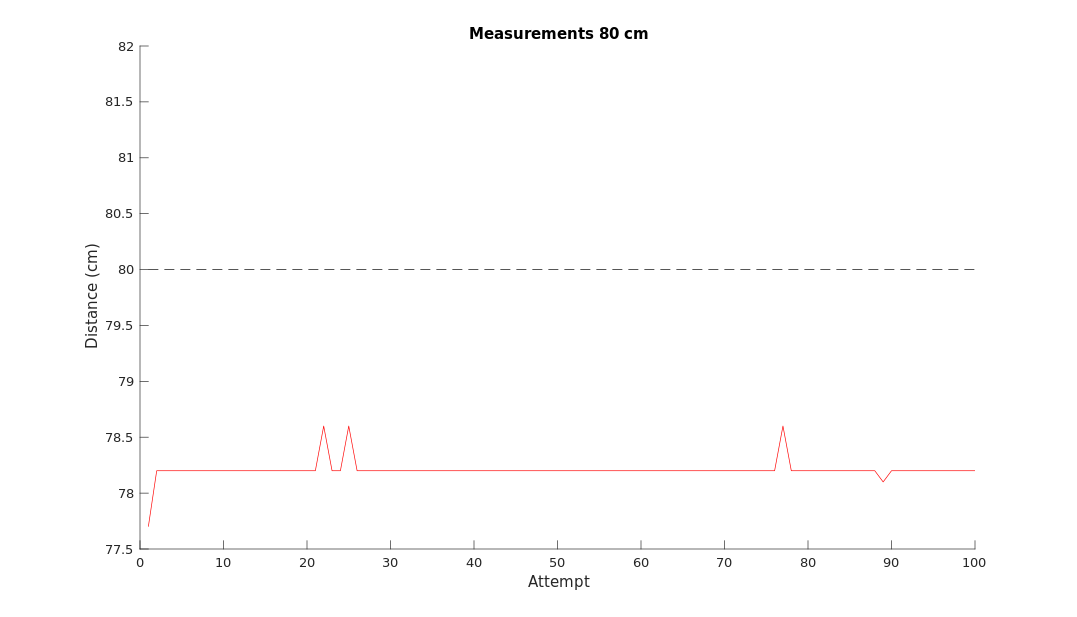
\includegraphics[width=\textwidth]{m80}
\end{figure}
\begin{figure}[H]
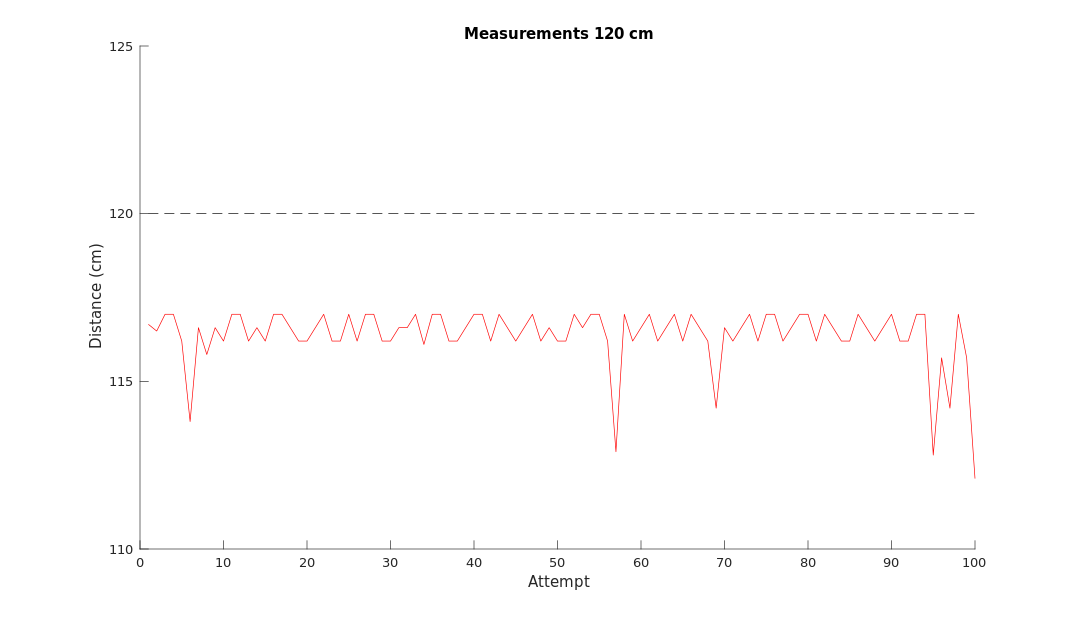
\includegraphics[width=\textwidth]{m120}
\end{figure}
\begin{figure}[H]
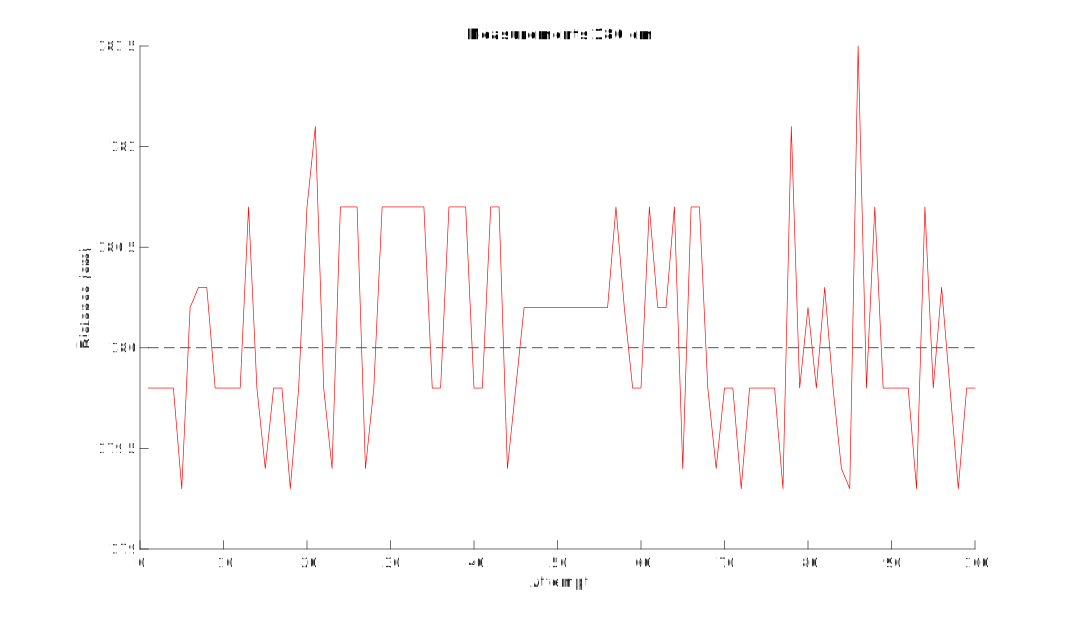
\includegraphics[width=\textwidth]{m180}
\end{figure}
\begin{figure}[H]
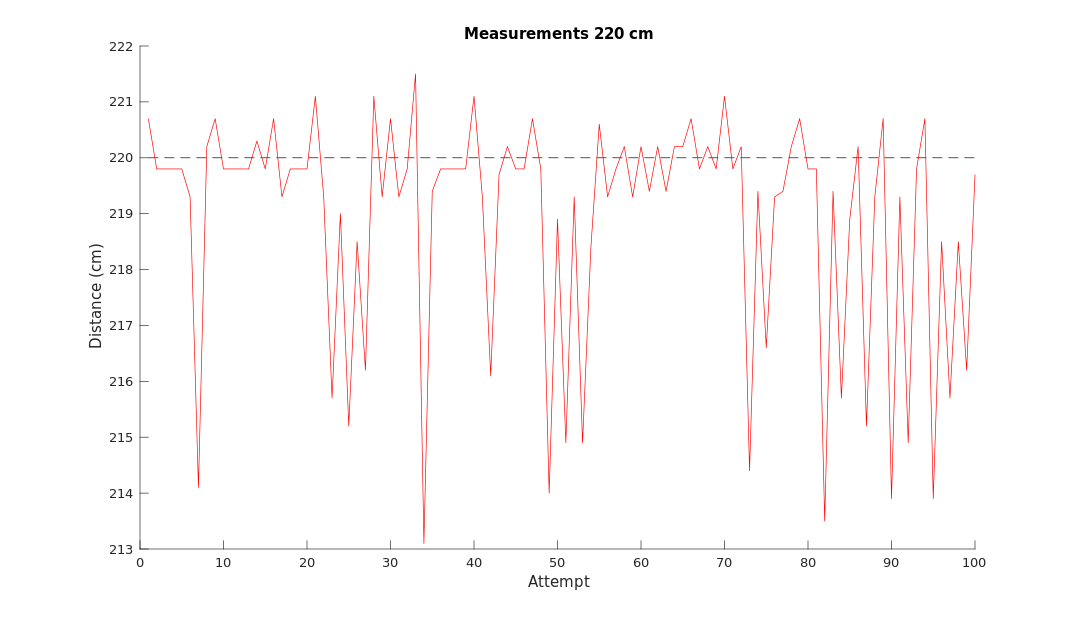
\includegraphics[width=\textwidth]{m220}
\end{figure}
\begin{figure}[H]
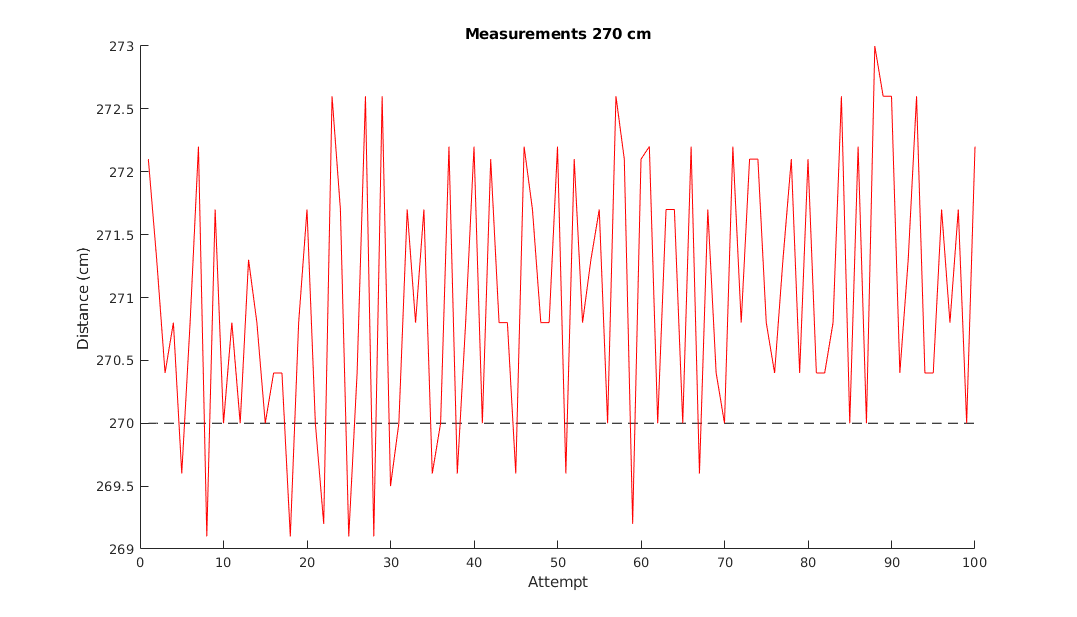
\includegraphics[width=\textwidth]{m270}
\end{figure}
\begin{figure}[H]
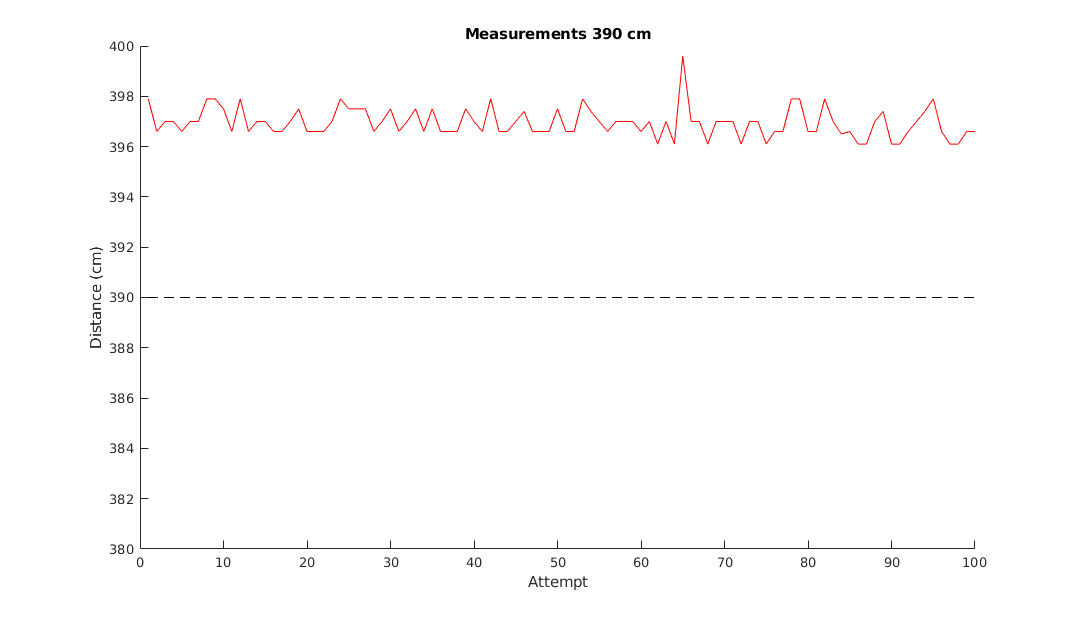
\includegraphics[width=\textwidth]{m390}
\end{figure}
\begin{center}
 \begin{tabular}{| c | c | c |} 
 \hline
 Distance & Mean & MSE\\ [0.5ex] 
 \hline\hline
 6 cm & 6.39 cm & 0.16 $cm^2$\\ 
 \hline
 10.5 cm & 10.90 cm &  0.25 $cm^2$\\
 \hline
 16 cm & 16.49 cm &  0.27 $cm^2$\\
 \hline
 20 cm& 20.30 cm& 0.10 $cm^2$\\
 \hline
 23 cm& 23.26 cm & 0.09 $cm^2$\\
 \hline
 60 cm& 61.05 cm & 1.25 $cm^2$ \\
 \hline
 80 cm& 78.20 cm & 3.22 $cm^2$ \\
 \hline
 120 cm& 116.38 cm & 13.83 $cm^2$ \\
 \hline
 150 cm& 135.53 cm& 446.26 $cm^2$\\
 \hline
 180 cm& 180.07 cm&  0.24 $cm^2$\\
 \hline
 220 cm& 218.92 cm&  5.36 $cm^2$\\
 \hline
 270 cm& 271 cm & 2.12 $cm^2$\\
 \hline
 390 cm& 396.95 cm & 2.12 $cm^2$\\ [1ex] 
 \hline
\end{tabular}
\end{center}
\newpage
\section{Conclusions and Future Works}
From the graphs we can see that the distance measurements, considering that during the tests some systemathic errors could have been made, are pretty accurate when the object is less than 2 meters away from the sensor. \\
Most of the errors and inaccuracies from the sensor can be associated with "noisy" environments and even to the inexpensiveness of the sensor.\\
Some of the possible future work on this project are to make this driver compatible with other microprocessors and try to solve some of the inaccuracies in the measurements. 